\documentclass{article}\usepackage[]{graphicx}\usepackage[]{color}
%% maxwidth is the original width if it is less than linewidth
%% otherwise use linewidth (to make sure the graphics do not exceed the margin)
\makeatletter
\def\maxwidth{ %
  \ifdim\Gin@nat@width>\linewidth
    \linewidth
  \else
    \Gin@nat@width
  \fi
}
\makeatother

\definecolor{fgcolor}{rgb}{0.345, 0.345, 0.345}
\newcommand{\hlnum}[1]{\textcolor[rgb]{0.686,0.059,0.569}{#1}}%
\newcommand{\hlstr}[1]{\textcolor[rgb]{0.192,0.494,0.8}{#1}}%
\newcommand{\hlcom}[1]{\textcolor[rgb]{0.678,0.584,0.686}{\textit{#1}}}%
\newcommand{\hlopt}[1]{\textcolor[rgb]{0,0,0}{#1}}%
\newcommand{\hlstd}[1]{\textcolor[rgb]{0.345,0.345,0.345}{#1}}%
\newcommand{\hlkwa}[1]{\textcolor[rgb]{0.161,0.373,0.58}{\textbf{#1}}}%
\newcommand{\hlkwb}[1]{\textcolor[rgb]{0.69,0.353,0.396}{#1}}%
\newcommand{\hlkwc}[1]{\textcolor[rgb]{0.333,0.667,0.333}{#1}}%
\newcommand{\hlkwd}[1]{\textcolor[rgb]{0.737,0.353,0.396}{\textbf{#1}}}%
\let\hlipl\hlkwb

\usepackage{framed}
\makeatletter
\newenvironment{kframe}{%
 \def\at@end@of@kframe{}%
 \ifinner\ifhmode%
  \def\at@end@of@kframe{\end{minipage}}%
  \begin{minipage}{\columnwidth}%
 \fi\fi%
 \def\FrameCommand##1{\hskip\@totalleftmargin \hskip-\fboxsep
 \colorbox{shadecolor}{##1}\hskip-\fboxsep
     % There is no \\@totalrightmargin, so:
     \hskip-\linewidth \hskip-\@totalleftmargin \hskip\columnwidth}%
 \MakeFramed {\advance\hsize-\width
   \@totalleftmargin\z@ \linewidth\hsize
   \@setminipage}}%
 {\par\unskip\endMakeFramed%
 \at@end@of@kframe}
\makeatother

\definecolor{shadecolor}{rgb}{.97, .97, .97}
\definecolor{messagecolor}{rgb}{0, 0, 0}
\definecolor{warningcolor}{rgb}{1, 0, 1}
\definecolor{errorcolor}{rgb}{1, 0, 0}
\newenvironment{knitrout}{}{} % an empty environment to be redefined in TeX

\usepackage{alltt}
\usepackage{graphicx}
\usepackage{hyperref}
\title{SOP 85: Using NOAA Climate Records}
\author{Marc Los Huertos and Isaac Medina}
\IfFileExists{upquote.sty}{\usepackage{upquote}}{}
\begin{document}
\maketitle

\section{Introduction}
Raw data sets often come with untidy/non-useful formats or information that must first be cleaned or processed before an accurate and useful analysis of the contents can be done. After obtaining a data set there are some preliminary steps you must follow in order to get your data file into working order for your analysis. 

\subsection{Purpose}
This document is intended as a resource and guide to help you: 
\begin{itemize}
\item upload your data file into the R environment using the Rstudio Server; and 
\item clean, organize and reformat the data to prepare it for analysis. 
\end{itemize}

The program that we will be using to run an analysis of our data is R, and we will access it via the Rstudio server using your computer's web browser. Essentially, we will be using computing software on the cloud to do our analysis so the first thing you will want know how to do is access the server. 

Note: Before you attempt to upload your data file into an appropriate directory in Rstudio you should already know how to access your Pomona Rstudio account as well as have connected to Marc's Github repository. Click on the following link to download a guide on how to get started with Rstudio and Github: \\
\\
\href{https://github.com/marclos/SOPs/raw/master/06_Rstudio_Github/Rstudio-and-Github_v03.pdf}{An Introduction to R, Rstudio, Github}

\section{Preparing CSV file(s)}



\subsection{Upload CSV Files into Appropriate Rstudio Directory} 
The first step to getting your data into R is to upload it into the the Rstudio server online. Follow these steps to upload your data file into an appropriate directory.\\ \emph{Note: following these steps requires you to be logged into an Rstudio account that is linked to Marc's repository, see above}

  \begin{enumerate}
  \item Once you're in Rstudio click on the folder entitled \textbf{``Climate\_Change\_Narratives"} in the \textit{Files} tab located in the lower right navigation block in Rstudio
  \item Navigate to a folder entitled \textbf{``Data"} 
  \item click on the correct folder for your class, it should correspond to the term in which you are enrolled in the EA 30 class. For example: SP17 if you're enrolled in EA 30 spring semester of 2017.
  \item Use the upload button to select a file from your computer to upload into the rstudio server
  \begin{figure}[h]
  \includegraphics[scale=0.25]{"/home/CAMPUS/im022012/Climate_Change_Narratives/graphics/Upload_button"}
  \end{figure}
  \item In the popup window select \textbf{Browse} and navigate to the climate data file you downloaded from the CDO website (SOP 84). Hopefully you still remember where you saved it and what name you saved it under. 
  \item Click \textbf{Open} and then click 
  
  \end{enumerate}




\subsection{Preprocessing CSV files}

In most cases, we don't need to preprocess the csv files. However, Mac users have been confronted with a host of problems that has something to do with how Macs format CSV files.\footnote{I will update this when I try using a Mac for this.}


\section{Reading CSV Files into R}

Although the csv file might be present in an Rstudio directory, it is not in the R environment. One way to confirm this is to look at the Rstudio window tab `Environment', where the file listed. 

To have the file in the R environment, we read the file using the \verb!read.csv()! function. The function is expecting the path and name of the file as an argument inside the perentecies, which is tough to type without making errors. 

\subsection{Assigning the File Path and Name}

Okay, now we know what the file name and path look like from the eyes of R. In this example, the path and filename is:

%\begin{verbatim}
%"/home/CAMPUS/mwl04747/github/Climate_Change_Narratives/Data/Los Angeles_878024.csv"
%\end{verbatim}

We could paste the whole mess into the \texttt{read.csv()} function. Okay, let's keep moving. Although R was able to see the file, we still don't have an object we can actually do something with. Instead, we merely printed it to the screen. However, you have not created an object yet. To do this you need to assign it a name. So, what do we need to make an object?  Yes, the name of the object and the use of the assignment symbol. Let's create an object names filename instead that has the whole path and file name in it. Start with the name you want to use before the \texttt{read.csv()} function like this:

First, we will import the CSV file. In most cases, we don't need to preprocess the csv files. Use "file.choose" to find the folder path name. 

We will use a pop-up window to select the file the first time and then we'll assign the file path and name to an object. 

\begin{verbatim}
> choose.file()
\end{verbatim}

Need an impage of the pop-up window...

\subsection{Reading a CSV File into a Dataframe}

%\begin{verbatim}
%import <- read.csv(filename)
%\end{verbatim}

\subsection{Importing CSV Files}


Importing Scripts

%file = "/home/CAMPUS/mwl04747/github/Climate_Change_Narratives/Data/Los Angeles_878024.csv"

import = read.csv(file)

\begin{knitrout}
\definecolor{shadecolor}{rgb}{0.969, 0.969, 0.969}\color{fgcolor}\begin{kframe}
\begin{alltt}
\hlcom{# Read CSV}

\hlstd{file} \hlkwb{=} \hlstr{"/home/CAMPUS/im022012/Climate_Change_Narratives/Data/Singapore_ClimateData.csv"}

\hlstd{import} \hlkwb{=} \hlkwd{read.csv}\hlstd{(file)}
\end{alltt}
\end{kframe}
\end{knitrout}

\subsection{Confirming the Proper Reading of the CSV file}

in R, no news is good news, in other words, if you don't get red colored text describing an error, the program did something -- but now we need to figure out if it did something useful!

We need to ensure the that imported file is what you expected and that it read the csv file correctly. There are several ways to accomplish this. We should inspect the first few observations, evaluate the structure of the dataframe and finally plot the data. We will do all of the these below.

\subsubsection{Viewing the 1st 6 Observations}

\begin{knitrout}
\definecolor{shadecolor}{rgb}{0.969, 0.969, 0.969}\color{fgcolor}\begin{kframe}
\begin{alltt}
\hlkwd{head}\hlstd{(import)}
\end{alltt}
\begin{verbatim}
##             STATION                      STATION_NAME     DATE     PRCP
## 1 GHCND:SNM00048698 SINGAPORE CHANGI INTERNATIONAL SN 19620512     0.16
## 2 GHCND:SNM00048698 SINGAPORE CHANGI INTERNATIONAL SN 19620516     0.08
## 3 GHCND:SNM00048698 SINGAPORE CHANGI INTERNATIONAL SN 19620605 -9999.00
## 4 GHCND:SNM00048698 SINGAPORE CHANGI INTERNATIONAL SN 19621006     0.39
## 5 GHCND:SNM00048698 SINGAPORE CHANGI INTERNATIONAL SN 19621007     0.02
## 6 GHCND:SNM00048698 SINGAPORE CHANGI INTERNATIONAL SN 19621012     0.08
##   TAVG  TMAX  TMIN
## 1   81 -9999    75
## 2   79    86    75
## 3   84    93    77
## 4   83    91 -9999
## 5   84    91    79
## 6   78    84 -9999
\end{verbatim}
\end{kframe}
\end{knitrout}

\subsubsection{Confirming the Column Names}

\begin{knitrout}
\definecolor{shadecolor}{rgb}{0.969, 0.969, 0.969}\color{fgcolor}\begin{kframe}
\begin{alltt}
\hlkwd{names}\hlstd{(import)}
\end{alltt}
\begin{verbatim}
## [1] "STATION"      "STATION_NAME" "DATE"         "PRCP"        
## [5] "TAVG"         "TMAX"         "TMIN"
\end{verbatim}
\end{kframe}
\end{knitrout}

\subsubsection{Evaluating the structure of the object}

Okay, you know have created a data frame. To confirm this, type \texttt{str(import)} and you should see some strange text that describes the data frame. This function allow you to peer into the data frame structure. You you see it is a data frame and it has several variables and each one has certain characteristics and R even shows you some of the observations. This is a good thing to get into the habitat of check, for you want to ensure the data have been imported in a way that you expect.


\begin{knitrout}
\definecolor{shadecolor}{rgb}{0.969, 0.969, 0.969}\color{fgcolor}\begin{kframe}
\begin{alltt}
\hlkwd{str}\hlstd{(import)}
\end{alltt}
\begin{verbatim}
## 'data.frame':	13704 obs. of  7 variables:
##  $ STATION     : Factor w/ 1 level "GHCND:SNM00048698": 1 1 1 1 1 1 1 1 1 1 ...
##  $ STATION_NAME: Factor w/ 1 level "SINGAPORE CHANGI INTERNATIONAL SN": 1 1 1 1 1 1 1 1 1 1 ...
##  $ DATE        : int  19620512 19620516 19620605 19621006 19621007 19621012 19621022 19621104 19621105 19621121 ...
##  $ PRCP        : num  0.16 0.08 -9999 0.39 0.02 ...
##  $ TAVG        : int  81 79 84 83 84 78 81 78 79 81 ...
##  $ TMAX        : int  -9999 86 93 91 91 84 91 88 91 -9999 ...
##  $ TMIN        : int  75 75 77 -9999 79 -9999 75 73 73 75 ...
\end{verbatim}
\end{kframe}
\end{knitrout}

Remember, a data frame is a set of vectors. To access the data inside the data frame, you can use the following command


\subsubsection{Plotting the Data}

Now we will check the data by plotting it (Figure~\ref{fig:plotmissing}).

\begin{figure}

\begin{knitrout}
\definecolor{shadecolor}{rgb}{0.969, 0.969, 0.969}\color{fgcolor}\begin{kframe}
\begin{alltt}
\hlkwd{plot}\hlstd{(TMAX}\hlopt{~}\hlstd{DATE, import)}
\end{alltt}
\end{kframe}
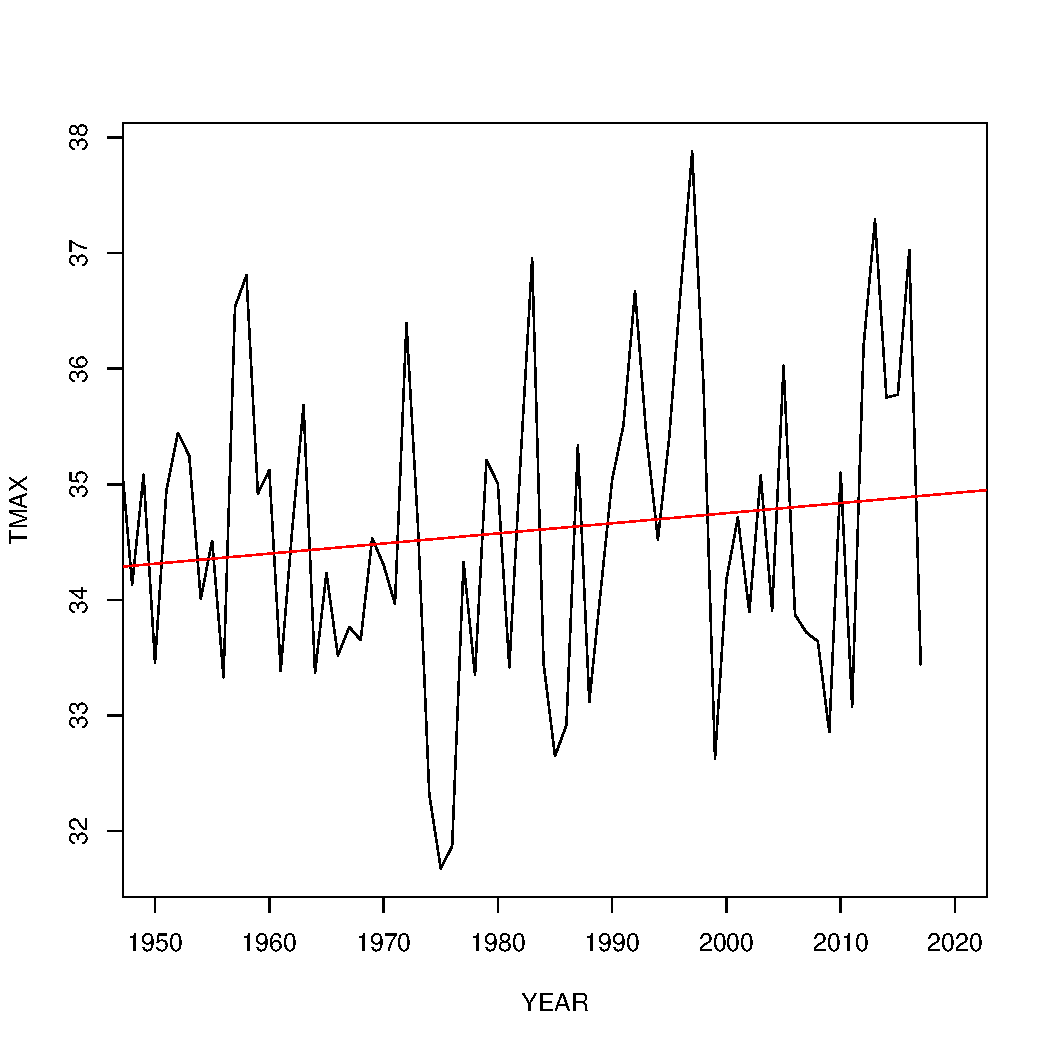
\includegraphics[width=\maxwidth]{figure/unnamed-chunk-5-1} 

\end{knitrout}
\caption{Some Caption.}
\label{fig:plotmissing}
\end{figure}

We find some rather odd low temperature values in the plot. We can find some of these with the \texttt{min()} function.

\begin{knitrout}
\definecolor{shadecolor}{rgb}{0.969, 0.969, 0.969}\color{fgcolor}\begin{kframe}
\begin{alltt}
\hlkwd{min}\hlstd{(import}\hlopt{$}\hlstd{TMAX)}
\end{alltt}
\begin{verbatim}
## [1] -9999
\end{verbatim}
\end{kframe}
\end{knitrout}

\subsection{Re-assigning Missing Values to NAs}

What's going on?  What is the deal with the -9999? These are used for missing data. Historically, computers didn't have a lot of options for mixing numbers and letters in a variable type while R has some built in flexibility for this. So, to avoid leaving values blank (with all the ambiguous interpretations), the value -9999 is used to sybmolize missing values, since the number is unrealistic in the real world!

Obviously, if we averaged the temperature with these values, we'd get a pretty inaccurate number (e.g. -3946 versus 89. Thus, we need to remove them!  

We will replace the -9999 with NA, which R uses specifically to avoid accidently averaging arbitrary values that are representing missing values. 

How do we do this?
\begin{knitrout}
\definecolor{shadecolor}{rgb}{0.969, 0.969, 0.969}\color{fgcolor}\begin{kframe}
\begin{alltt}
\hlstd{import}\hlopt{$}\hlstd{TMAX[import}\hlopt{$}\hlstd{TMAX}\hlopt{==-}\hlnum{9999}\hlstd{]} \hlkwb{=} \hlnum{NA}
\hlstd{import}\hlopt{$}\hlstd{TMIN[import}\hlopt{$}\hlstd{TMIN}\hlopt{==-}\hlnum{9999}\hlstd{]} \hlkwb{=} \hlnum{NA}
\end{alltt}
\end{kframe}
\end{knitrout}


Okay, now we'll check again, but let's plot a just a few years, let's say five years (356 days * 5 years = 1825) or 1825 observations. 

\begin{knitrout}
\definecolor{shadecolor}{rgb}{0.969, 0.969, 0.969}\color{fgcolor}\begin{kframe}
\begin{alltt}
\hlkwd{plot}\hlstd{(TMAX}\hlopt{~}\hlstd{DATE, import[}\hlnum{1}\hlopt{:}\hlnum{1835}\hlstd{,],} \hlkwc{ty}\hlstd{=}\hlstr{'l'}\hlstd{)}
\end{alltt}
\end{kframe}
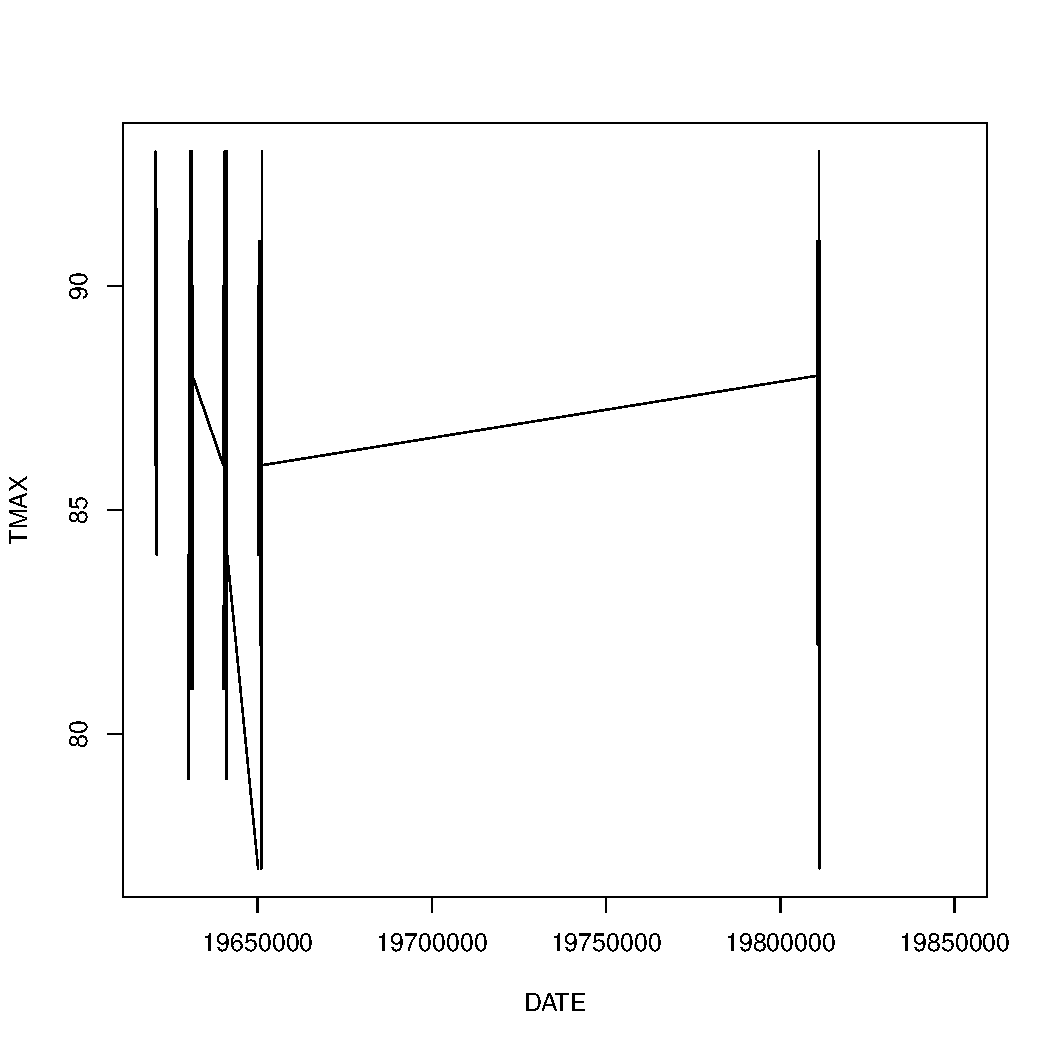
\includegraphics[width=\maxwidth]{figure/unnamed-chunk-8-1} 

\end{knitrout}

Yikes! What's wrong? It appears we have gaps in the data -- but we already removed our missing data, why are these big jumps in the data. 

As it turns out the problem is that with how the dates are specified. In particular, the Dec 31 to Jan 1 transition. Let's say that the data have a year change between 1913 and 1914. The date format in the NOAA data are YYYYMMDD, or year, month, and day with 4, 2, 2 digits, respectively. Thus, the last day of 1913 is 19131231 or Dec, 31, 1913. The next day is January 1st or 19140101. But when you plot these on the x-axis, the order of the values should be $19131231 \rightarrow 19131232 \rightarrow 19131233 \rightarrow 19131234$, etc but there is no 32nd, 33rd or 34th of December. Instead the dates go from  $19131231 \rightarrow 19140101$. We have lots of numbers that are skipped, but no coded as missing, but missing all the same. So, now we need to convert our dates to something more sensible. In R, that means creating a variable with a format that expects dates, thus doesn't plot numbers that are impossible dates!

\subsection{Converting Date Format}

To create a new format, we have to complete a few steps. Unfortunately, date formats are one of the more obtuse aspects of R, but if you follow along, you should have success, even if you have no clue what you did. 
First, we convert the date to a string of character values. Next, we'll convert the strings to a data format. 

\begin{knitrout}
\definecolor{shadecolor}{rgb}{0.969, 0.969, 0.969}\color{fgcolor}\begin{kframe}
\begin{alltt}
\hlstd{strDates} \hlkwb{<-} \hlkwd{as.character}\hlstd{(import}\hlopt{$}\hlstd{DATE)}
\hlkwd{head}\hlstd{(strDates)}
\end{alltt}
\begin{verbatim}
## [1] "19620512" "19620516" "19620605" "19621006" "19621007" "19621012"
\end{verbatim}
\begin{alltt}
\hlstd{import}\hlopt{$}\hlstd{NewDate} \hlkwb{<-} \hlkwd{as.Date}\hlstd{(strDates,} \hlstr{"%Y%m%d"}\hlstd{)}
\end{alltt}
\end{kframe}
\end{knitrout}

\subsection{Checking the New Dates}

\begin{knitrout}
\definecolor{shadecolor}{rgb}{0.969, 0.969, 0.969}\color{fgcolor}\begin{kframe}
\begin{alltt}
\hlkwd{plot}\hlstd{(TMAX}\hlopt{~}\hlstd{NewDate, import[}\hlnum{1}\hlopt{:}\hlnum{1835}\hlstd{,],} \hlkwc{ty}\hlstd{=}\hlstr{'l'}\hlstd{)}
\end{alltt}
\end{kframe}
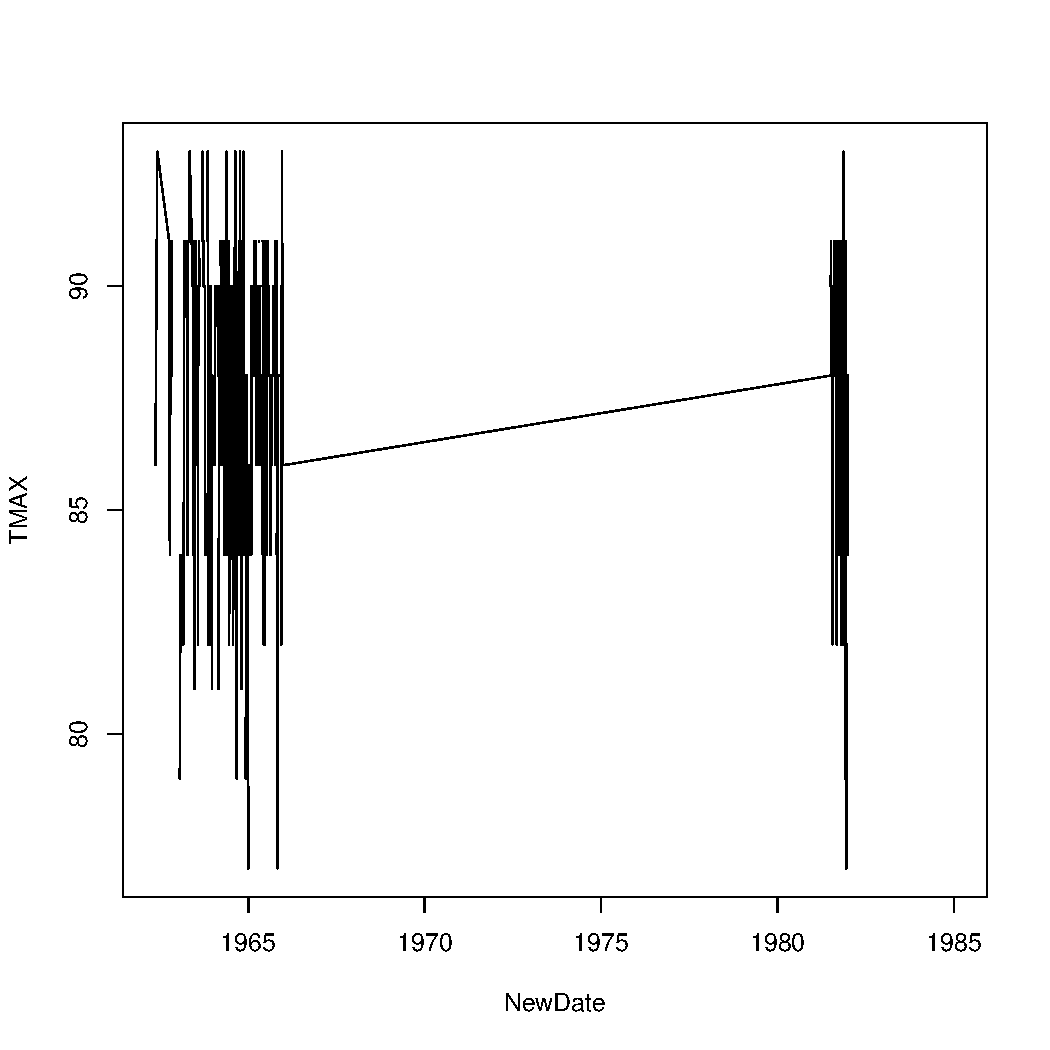
\includegraphics[width=\maxwidth]{figure/unnamed-chunk-10-1} 

\end{knitrout}

%\subsection{Subset Sites}

%unique(import$STATION_NAME)
%Let's choose the FAIRPLEX NY US because the record is longer than the airport.

%LosAngeles <- subset(import, STATION_NAME=="LOS ANGELES DOWNTOWN USC CA US", select=c(STATION, STATION_NAME, DATE, NewDate, TMIN, TMAX, PRCP))


%plot(TMAX~NewDate, LosAngeles, ty='l')





\begin{knitrout}
\definecolor{shadecolor}{rgb}{0.969, 0.969, 0.969}\color{fgcolor}\begin{kframe}
\begin{alltt}
\hlcom{#maunaloa$average}
\end{alltt}
\end{kframe}
\end{knitrout}

to dump the average CO$_2$ concentrations readings onto your screen as a vector. You should see some ~627 observations, depending on how recent the data have been uploaded. So, the dollar symbol is used to drill into the data frame vectors.  And when you look at the \texttt{str()} function again, you will see these dollar signs again.

\section{Preparing Records for Analysis}





\end{document}
